In this section I'm going to first introduce what Protocol Buffers are.
Then, I'm going to analyze existing solutions of website documentations with the ability to call APIs for Protocol Buffers, GraphQL and RESTful APIs.
I'll start with Protocol Buffers, then I'll move and explore the solutions to GraphQL and finally I'll analyze RESTful API\@.


\section{Protocol Buffers}
Protocol Buffers are a mechanism for serializing structured data.
The are language-neutral and platform-neutral.
They encompass:
\begin{itemize}
    \item definition language,
    \item compiler-generated code,
    \item language-specific runtime libraries,
    \item serialization format.
\end{itemize}
The definition language is used to define data structures, expressed in .proto files.
The compiler-generated code is used to enable interaction with the defined data structures in a specific programming language.
The language-specific runtime libraries are used to facilitate the serialization and deserialization of data according to the Protocol Buffer format.
The serialization format is a compact binary format used for storing Protocol Buffer data in files or transmitting it across network connections.
\cite{protobuf-overview}

The mechanism of typical workflow is described in the figure~\ref{fig:protobuf-mechanism}.
For the purpose of this work, my main focus will be on generating the code from the .proto files and using the generated code to interact with the final APIs.
\begin{figure}[hbt!]
    \centering
    \captionsetup{justification=centering}
    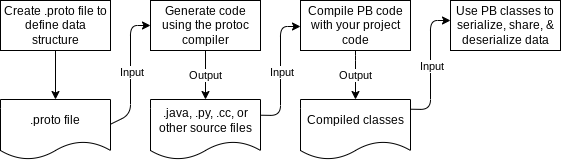
\includegraphics[width=0.8\textwidth]{images/protocol-buffers-concepts.png}
    \caption{Protocol Buffers Workflow~\cite{protobuf-overview}}
    \label{fig:protobuf-mechanism}
\end{figure}

There are two language versions of Protocol Buffers, version 2 and version 3.
The versions share the same basic concepts, use the same syntax, but version 3 improves on version 2 in several ways~\cite{protobuf-proto3}.
As this work is focused on the latest technologies, I will be focusing on version 3 of Protocol Buffers.
If no specific version is mentioned, it is assumed that version 3 is used.

\subsection{Types}
The basic keywords in Protocol Buffers are \textit{message}, \textit{enum}, \textit{service}, \textit{method} and \textit{package}.
The \textit{message} is used to define a data structure.
The \textit{enum} is used to define a set of named constants.
The \textit{service} is set of \textit{methods} that can be called remotely.
And, the \textit{package} type is used to define a namespace for the defined \textit{messages}, \textit{enums} and \textit{services}.
\cite{protobuf-proto3}

\subsubsection{Message}
Messages are used to define data structures.
They are defined using the \textit{message} keyword followed by the name of the message and a block of fields.
Each field has a name, a type and a unique number (it doesn't have to be defined manually).
The type of a field can be a scalar type or another message type.

% The scalar types are described in the table~\ref{tab:protobuf-scalar-types}.

% Numbering
% Repeated
% Map
% Optional
% One Of
% Options

\cite{protobuf-proto3}

\subsubsection{Enum}

\subsubsection{Method}

\subsection{Comments}

\subsection{Code Generation}


\section{Website Documentation}

\subsection{Protocol Buffers}

\subsection{GraphQL}

\subsection{RESTful API}

\subsection{Summary}

\subsection{Issues}


\section{Requirements}
On the basis of the previously described problems and main requirements, I have compiled functional and non-functional requirements covering the required functionality of the static web generator.

\subsection{Functional}
% Co má systém umět

%\subsubsection{F1 -- Pomocník pro inicializaci obrazu softwaru Syllabus Plus}
%Pro inicializaci obrazu softwaru Syllabus Plus a další práci s daty je potřeba zadat informace o daném semestru.
%Správné nastavení je klíčové pro korektní plánování časových lístků.

\subsection{Non-Functional}

%\subsubsection{N1 -- Aplikace s grafickým uživatelským rozhraním}
%Aplikace by měla mít grafické uživatelské rozhraní pro práci s daty.
%Uživatel by tak měl být schopen obsluhovat aplikaci sám bez pomoci další osoby.


\section{Use Cases}


%\begin{figure}
%    \centering
%    \captionsetup{justification=centering}
%    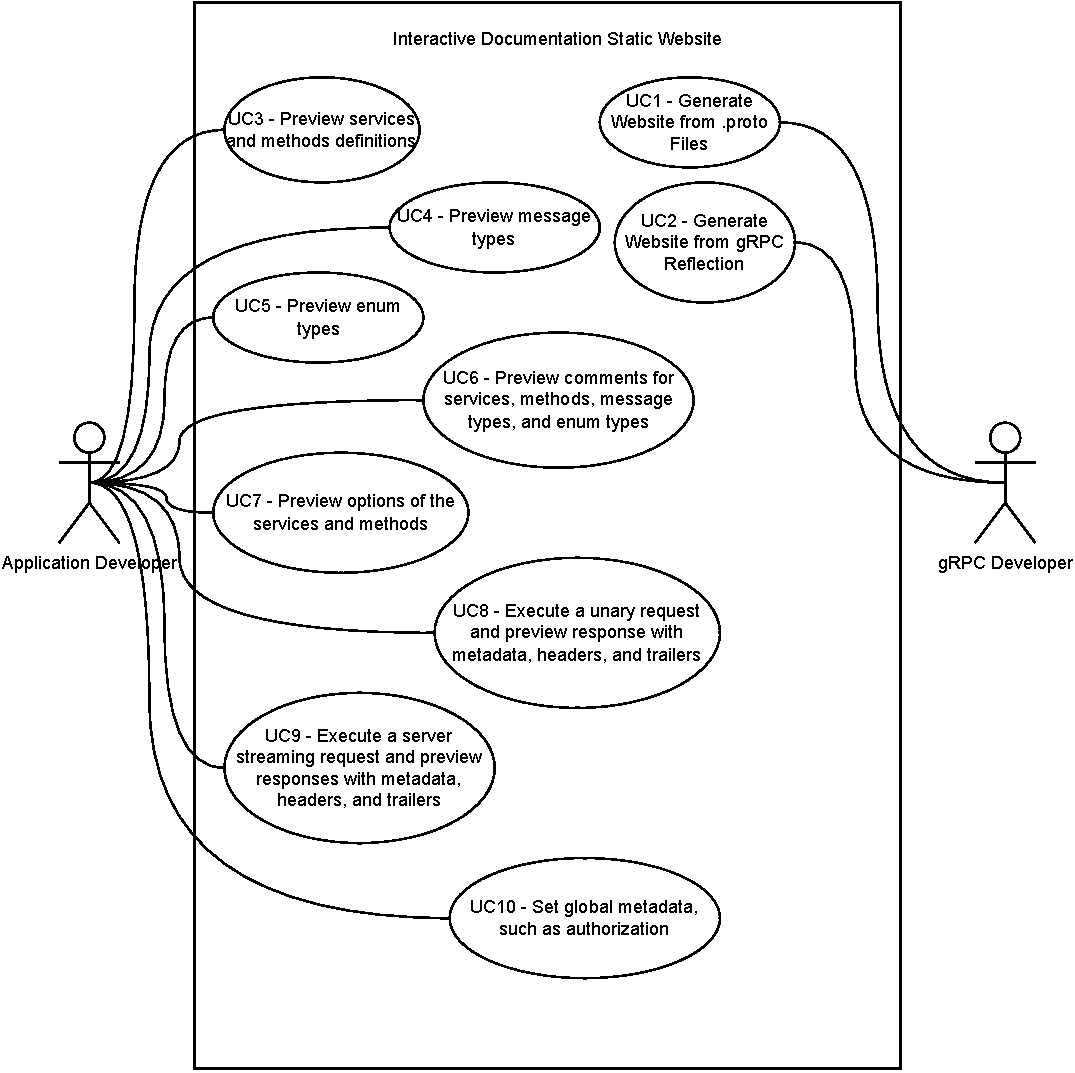
\includegraphics[width=1.0\textwidth]{use-case-diagram}
%    \caption{Diagram případů užití}
%    \label{fig:use-case-diagram}
%\end{figure}

%\subsection{UC1 -- Inicializace obrazu softwaru Syllabus Plus}
%Rozvrhář spustí software Syllabus Plus a začne s inicializací nového obrazu.
%Během inicializace se mu zobrazí dialog pro nastavení začátku semestru, vyučované dny, začátek a konec hodin, počet hodin za den a počet týdnů na semestr.
%Rozvrhář otevře aplikaci pro převod a nastaví semestr, který se využije pro načítání dat ze systému KOS\@.
%Zobrazí si jakým způsobem má položky nastavit, aby byla data správně reprezentována (například při plánování časových lístků).
%Formulář vyplní podle získaných dat z aplikace a inicializuje obraz.
%V případě, že se rozvrhář splete, musí aktuální obraz smazat a začít vytvářet nový od začátku.
%Jinak je inicializace úspěšně dokončena.


\section{Requirements to Use Cases Mapping}
I have compiled a table of requirements and use cases mapping (see table~\ref{tab:use_cases}) to verify that all requirements are covered by at least one use case and that no use case is unnecessary.
The table shows that all requirements are covered.

\begin{table}[hbt!]
    \centering
    \captionsetup{justification=centering}
    \begin{tabular}{|l|l|l|l|l|l|l|l|l|l|l|l|l|l|l|l|}
        \hline
        & \multicolumn{15}{c|}{Use Cases} \\ \hline
        & 1 & 2 & 3 & 4 & 5 & 6 & 7 & 8 & 9 & 10 & 11 & 12 & 13 & 14 & 15 \\ \hline
        F1  & x &   &   &   &   &   &   &   &   &    &    &    &    &    &    \\ \hline
        F2  &   &   & x &   &   &   &   &   &   &    &    &    &    &    &    \\ \hline
        F3  &   &   &   & x &   &   &   &   &   &    &    &    &    &    &    \\ \hline
        F4  &   &   &   &   &   &   &   &   &   &    &    &    &    &    & x  \\ \hline
        F5  &   &   &   &   & x &   &   &   &   &    &    &    &    &    &    \\ \hline
        F6  &   & x &   &   &   &   &   & x &   &    &    & x  & x  &    &    \\ \hline
        F7  &   & x &   &   &   &   &   &   &   &    &    & x  &    &    &    \\ \hline
        F8  &   &   &   &   &   &   &   &   &   &    &    &    & x  &    &    \\ \hline
        F9  &   & x &   &   &   &   &   &   &   &    & x  &    &    &    &    \\ \hline
        F10 &   & x &   &   &   &   &   &   &   &    &    &    &    &    &    \\ \hline
        F11 &   &   &   &   &   &   &   &   & x & x  &    &    &    &    &    \\ \hline
        F12 &   & x &   &   &   &   &   &   &   &    &    &    &    &    &    \\ \hline
        F13 &   &   &   &   &   &   &   &   &   & x  &    &    &    &    &    \\ \hline
        F14 &   &   &   &   &   &   &   & x & x & x  &    & x  & x  &    &    \\ \hline
        F15 &   &   &   &   &   &   &   & x & x & x  &    & x  &    &    &    \\ \hline
        F16 &   &   &   &   &   &   &   & x & x & x  &    & x  & x  &    &    \\ \hline
        F17 &   &   &   &   &   & x & x &   &   &    &    &    &    &    &    \\ \hline
        F18 &   &   &   &   &   & x &   &   &   & x  &    &    &    & x  &    \\ \hline
        F19 & x &   &   &   &   &   &   &   &   &    &    &    &    &    &    \\ \hline
    \end{tabular}
    \caption{Requirements to Use Cases Mapping}
    \label{tab:use_cases}
\end{table}